\let\negmedspace\undefined
\let\negthickspace\undefined
\documentclass[journal]{IEEEtran}
\usepackage[a5paper, margin=10mm, onecolumn]{geometry}
%\usepackage{lmodern} % Ensure lmodern is loaded for pdflatex
\usepackage{tfrupee} % Include tfrupee package

\setlength{\headheight}{1cm} % Set the height of the header box
\setlength{\headsep}{0mm}     % Set the distance between the header box and the top of the text
\usepackage{gvv-book}
\usepackage{gvv}
\usepackage{cite}
\usepackage{amsmath,amssymb,amsfonts,amsthm}
\usepackage{algorithmic}
\usepackage{graphicx}
\usepackage{textcomp}
\usepackage{xcolor}
\usepackage{txfonts}
\usepackage{listings}
\usepackage{enumitem}
\usepackage{mathtools}
\usepackage{gensymb}
\usepackage{comment}
\usepackage[breaklinks=true]{hyperref}
\usepackage{tkz-euclide} 
\usepackage{listings}
% \usepackage{gvv}                                        
\def\inputGnumericTable{}                                 
\usepackage[latin1]{inputenc}                                
\usepackage{color}                                            
\usepackage{array}                                            
\usepackage{longtable}                                       
\usepackage{calc}                                             
\usepackage{multirow}                                         
\usepackage{hhline}                                           
\usepackage{ifthen}                                           
\usepackage{lscape}
\begin{document}

\bibliographystyle{IEEEtran}
\vspace{3cm}

\title{3.3.1}
\author{EE24BTECH11030 - J.KEDARANANDA}
% \maketitle
% \newpage
% \bigskip
{\let\newpage\relax\maketitle}

\renewcommand{\thefigure}{\theenumi}
\renewcommand{\thetable}{\theenumi}
\setlength{\intextsep}{10pt} % Space between text and floats


\numberwithin{equation}{enumi}
\numberwithin{figure}{enumi}
\renewcommand{\thetable}{\theenumi}


\textbf{Question}:\\
Draw a  $\triangle ABC$ with $\boldsymbol{BC} = 6 \text{ cm}$, $\boldsymbol{AB} = 5 \text{ cm}$, and $\angle B = 60^\circ$.
\\ \solution \\
    \begin{table}[h!]    
      \centering
      \begin{center}
    \begin{tabular}{|c|c|} 
        \hline
            \textbf{Variable} & \textbf{Value} \\ 
        \hline
            $\boldsymbol{BC}$ & 6 cm \\ 
        \hline
            $\boldsymbol{AB}$ & 5 cm \\ 
        \hline
            $\angle \vec{B}$  & $60^\circ$ \\
        \hline
    \end{tabular}
\end{center}  



      \caption{}
    \end{table}\\
We need to find b. Using the Law of Cosines, we have:
\begin{align}
    b^2 &= c^2 + a^2 - 2ca \cos(B) \\
    b^2 &= 5^2 + 6^2 - 2 \cdot 5 \cdot 6 \cdot \cos(60^\circ) \\
    &= 25 + 36 - 2 \cdot 5 \cdot 6 \cdot \frac{1}{2} \\
    &= 25 + 36 - 30 \\
    &= 31 \\
    \boldsymbol{AC} &= \sqrt{31} \approx 5.57 \, \text{cm}
\end{align}

Thus, the length of side  $\boldsymbol{AC}$  is approximately 5.57  $\text{cm}$ .

    \begin{figure}[h]
       \centering
       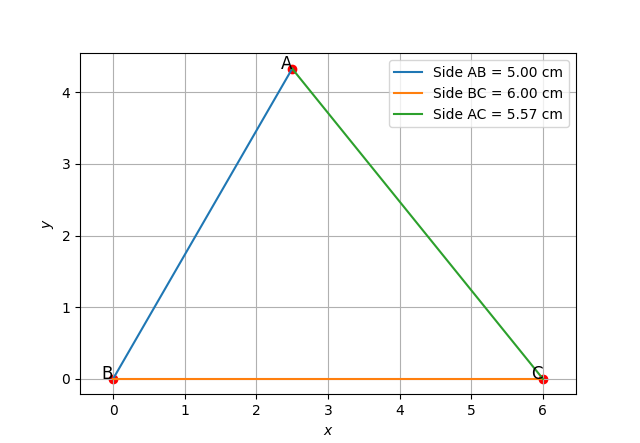
\includegraphics[width=\linewidth]{figs/fig1.png}
       \caption{}
       \label{graph}
    \end{figure}
\end{document}  









